% ****** Start of file apssamp.tex ******
%
%   This file is part of the APS files in the REVTeX 4.2 distribution.
%   Version 4.2a of REVTeX, December 2014
%
%   Copyright (c) 2014 The American Physical Society.
%
%   See the REVTeX 4 README file for restrictions and more information.
%
% TeX'ing this file requires that you have AMS-LaTeX 2.0 installed
% as well as the rest of the prerequisites for REVTeX 4.2
%
% See the REVTeX 4 README file
% It also requires running BibTeX. The commands are as follows:
%
%  1)  latex apssamp.tex
%  2)  bibtex apssamp
%  3)  latex apssamp.tex
%  4)  latex apssamp.tex
%
\documentclass[%
 reprint,
superscriptaddress,
%groupedaddress,
%unsortedaddress,
%runinaddress,
%frontmatterverbose, 
%preprint,
%preprintnumbers,
%nofootinbib,
%nobibnotes,
%bibnotes,
 amsmath,amssymb,
 aps,
%pra,
%prb,
%rmp,
%prstab,
%prstper,
%floatfix,
]{revtex4-2}

\usepackage{graphicx}% Include figure files
\usepackage{dcolumn}% Align table columns on decimal point
\usepackage{bm}% bold math
\usepackage{hyperref}% add hypertext capabilities
\usepackage{physics} % for \ket and other quantum notation
\usepackage{amsthm}
%\usepackage[mathlines]{lineno}% Enable numbering of text and display math
%\linenumbers\relax % Commence numbering lines

%\usepackage[showframe,%Uncomment any one of the following lines to test 
%%scale=0.7, marginratio={1:1, 2:3}, ignoreall,% default settings
%%text={7in,10in},centering,
%%margin=1.5in,
%%total={6.5in,8.75in}, top=1.2in, left=0.9in, includefoot,
%%height=10in,a5paper,hmargin={3cm,0.8in},
%]{geometry}
\newtheorem{theorem}{Theorem}[section]
\newtheorem{corollary}{Corollary}[theorem]
\newtheorem{lemma}[theorem]{Lemma}
\newtheorem{definition}{Definition}[section]

\DeclareRobustCommand{\bbone}{\text{\usefont{U}{bbold}{m}{n}1}}

\DeclareMathOperator{\EX}{\mathbb{E}}% expected value

\begin{document}

\preprint{APS/123-QED}

\title{One-way Symmetric Private Information Retrieval Protocol with One Single Database Achieving Statistical Security}% Force line breaks with \\

\author{Xiang Zou}
\email{xiang.zou@mail.utoronto.ca}
\thanks{These authors contributed equally to this work.}
\affiliation{%
 Department of Physics, University of Toronto, 60 St. George Street, Toronto, ON, M5S 1A7, Canada
}%

 %\altaffiliation[Also at ]{Physics Department, XYZ University.}%Lines break automatically or can be forced with \\
\author{Hoi Fung Chau}
\email{hfchau@hku.hk}
\thanks{These authors contributed equally to this work.}
\affiliation{%
 Department of Physics, The University of Hong Kong, Pokfulam Road, Hong Kong Island, Hong Kong
}%



\date{\today}% It is always \today, today,
             %  but any date may be explicitly specified

\begin{abstract}
In this paper, we investigate a possible protocol to achieve Symmetric Private Information Retrieval with one-way QKD and one single database.
\end{abstract}

%\keywords{Suggested keywords}%Use showkeys class option if keyword%display desired
\maketitle

%\tableofcontents

\section{Introduction}

Secure access to remote databases is a central primitive in both classical and quantum cryptography~\cite{QPQ1, QPQ2, QPQ3, QSPIR_multiple_database1, QSPIR_multiple_database2, Insecurity_Quantum_Oblivious_transfer1}, with applications ranging from cloud storage and biometric identification to distributed ledgers and secure multiparty computation. In this context, private information retrieval (PIR) allows a client to retrieve partial data from a database held by a server without revealing which item was requested, thereby protecting the privacy of the client’s query. While Symmetric private information retrieval (SPIR) strengthens this notion by additionally requiring database privacy, the client must not learn anything about the database beyond the requested item, even if the client is computationally unbounded~\cite{QSPIR_theory1, QSPIR_multiple_database1, QSPIR_multiple_database2, SPIR1, SPIR2, SPIR3}.

Classical PIR and SPIR have been extensively studied before~\cite{PIR1, PIR2, PIR3, SPIR1, SPIR2, SPIR3}. In the information-theoretic setting, it is by now well understood that single-server PIR and SPIR suffer from strong limitations in classical communication: if only one database server is available and no computational assumptions are made, then any PIR scheme with perfect user privacy must reveal essentially the entire database to the user, and information-theoretic SPIR with a single database server is impossible except for the trivial protocol where the entire database is sent~\cite{PIR1, PIR2}.


To obtain nontrivial communication complexity and database privacy, classical SPIR protocols assume either multiple non-communicating database servers that share randomness, or they rely on computational hardness assumptions such as the hardness of lattice or number-theoretic problems~\cite{SPIR1, SPIR2, SPIR3}.

These multi-server SPIR protocols can achieve sublinear communication complexity~\cite{SPIR1, SPIR2, SPIR3} and strong security guarantees, but they require architectural assumptions—such as multiple independent data centers and pre-distributed shared randomness—that may be difficult or costly to realize in practice, if not impossible.

Quantum communication offers new tools to revisit PIR and SPIR. Genuinely quantum protocols can outperform classical ones in certain regimes: for example, quantum symmetrically-private information retrieval (QSPIR) schemes achieve sublinear communication with multiple servers and no shared randomness~\cite{QSPIR_multiple_database1, QSPIR_multiple_database2}, while still protecting both user and database privacy against honest-but-curious participants.

A parallel line of work on quantum private queries (QPQ) has proposed cheat-sensitive protocols~\cite{QPQ1, QPQ2, QPQ3} in which a single quantum server can answer private queries to a classical database with strong user privacy and bounded database leakage per query, at the price of relaxing full information-theoretic guarantees and allowing detection of server misbehaviour instead of preventing a third-party eavesdropper.

More recently, quantum-key-distribution (QKD)-assisted SPIR protocols and experimental demonstrations~\cite{QSPIR_multiple_database1, QSPIR_multiple_database2} have shown that quantum networks can be leveraged to distribute the secret keys and shared randomness needed for multi-database SPIR, but these schemes still fundamentally rely on multiple non-colluding databases or trust in specific network assumptions.

Despite this progress, the status of fully symmetric, information-theoretic private information retrieval from a single classical database remains unclear in the quantum setting. Existing negative results show that, under natural correctness and privacy requirements, perfect single-database SPIR is impossible even when quantum communication is allowed~\cite{Insecurity_Quantum_Oblivious_transfer1}, mirroring the classical impossibility of information-theoretic single-server SPIR.

In this work, a one-way quantum-communication protocol is presented that realizes symmetric private information retrieval between a single client and a single classical database server in an information-theoretic setting with statistical security.
The protocol uses a prepare-and-measure QKD-type architecture in which Bob, with a database, sends single-photon polarization states drawn from the BB84 alphabet to Alice, who is interested in parts of the database, over a one-way quantum channel, followed by classical post-processing over an authenticated classical public channel.

Operationally, the proposed protocol is attractive in that it uses only standard BB84-type sources and measurements, together with classical permutation, error correction, and privacy amplification, all of which are well within the reach of current QKD technology~\cite{Experimental_QKD1}. The one-way nature of the quantum communication, together with the fact that only a single database server is required, makes the architecture conceptually simple and directly compatible with existing quantum-communication links between a client and a data center.

This work thus provides a concrete candidate for achieving SPIR with one client, one classical database, and one-way quantum communication, together with explicit resource trade-offs between the database size, the block length, the unambiguous discrimination success probability, and the tolerated quantum bit error rate.


\section{Problem Statement}
\subsection{Description}

First, we quote the problem statement of SPIR, and clearly list out the assumptions in our setup.

Suppose there are two parties, Alice and Bob, and they have access to quantum communication channels and classical communication channels. Bob holds a private classical database with $n$ bits of data. Alice would like to find out the $i$-th bit of the database. In normal information retrieval process, Alice sends Bob a request for the $i$-th bit, and Bob responds. 

Apart from Alice and Bob, there exists an all-powerful third party, Eve, who has full control over whatever classical and quantum channels between Alice and Bob.

Upon the completion of the Information Retrieval process, we would like the scheme to achieve the following 3 goals (the walking definition of SPIR).

\begin{enumerate}
    \item No information is leaked to Eve.

    \item Bob has no idea which bit of information Alice wants to get.

    \item Alice can only get the bits of information she wants.
\end{enumerate}

\subsection{Formal Definition}
\label{sec:formal_definition}

Let $\Sigma=\{0, 1\}$. Suppose Bob holds a bit-string $\textbf{x}=\{x_0, x_1, \cdots, x_n\}\in\Sigma^n$ from an distribution $X$, and Alice is interested in bit $i$. 

We will demonstrate the existence of an approximate SPIR protocol with statistical security that utilizes a one-way quantum channel from Bob to Alice, along with public broadcasting channels accessible to both Alice and Bob, by employing some additional resources, the protocol will be largely similar to a QKD set up. After the protocol, Alice will possess a bit-string \( \mathbf{y} = \{y_0, y_1, \cdots, y_n\} \in \{0, 1\}^n \) derived from a distribution \( Y \), where \( x_i = y_i \). Additionally, denote the remaining bit strings \( \mathbf{x'} = \{x_0, \cdots, x_{i-1}, x_{i+1}, \cdots, x_n\} \) and \( \mathbf{y'} = \{y_0, \cdots, y_{i-1}, y_{i+1}, \cdots, y_n\} \), there exists, for an arbitrarily small \( \epsilon > 0 \), a resource measure such that \( I(\mathbf{x'}, \mathbf{y'}) \le \epsilon \). This ensures that Alice gains asymptotically no information about Bob beyond the specific bit of interest.

\section{The Protocol}
\label{sec:the_protocol}
In this section, we will describe the protocol that Alice and Bob use to achieve SPIR, the quantitative analysis will be discussed in later sections. This work is inspired of different well-studied QKD protocols in the prepare and measure scheme, where Bob prepares one of the four states, $\ket{0}, \ket{1}, \ket{+}, \ket{-}$, in photonic set up, it may represent the 4 polarizations of the photons, Horizontal, Vertical, Diagonal, and Anti-diagonal, respectively. Whereby convention, $\ket{0}, \ket{+}$ represent the physical bits $0$ in the $\sigma_Z$ and $\sigma_X$ basis respectively with a $+1$ eigenvalue; then, $\ket{1}, \ket{-}$ represent the physical bits $1$ in their respective basis with a $-1$ eigenvalue.

Bob holds a database of $n$ bits of data. Bob and Alice will collectively come up with an integer $k$, where they aim at achieving a length $kn$ physical bits at the end. The reason for needing the parameter $k$ will be clear in step 7. Meanwhile, they will agree on 2 other integers $m$ and $h'$; their usage will be explained later. 

\begin{enumerate}

    \item Bob randomly prepares one of the four states, $\ket{0}, \ket{1}, \ket{+}, \ket{-}$, and sends it to Alice. Alice acknowledges receipt and chooses a random basis (either $\sigma_Z$ or $\sigma_X$) to measure the state. Alice marks down both the chosen basis and the measurement result. The process is repeated until $kn+m+h'$ qubits are received by Alice.

    \item Alice and Bob use $m$ received states to estimate the error, where Bob and Alice collectively pick $m$ states that they will publicly announce the measurement basis and result, and then, they estimate both the bit flip and phase flip errors that occurred in the channel; if the error rate is too high, they abort the protocol; otherwise, they proceed. This error estimation step is to ensure that the eavesdropper gains no information; theoretical analysis is in section~\ref{sec:Security_against_Eve}, then they calculate the QKD key rate, denoted by $r$.

    \item For the remaining $kn+h'$ states, they will use $h'$ qubits to perform a normal QKD process (i.e., publicly announce the basis and discard the mismatched ones, then do error-correction and privacy amplification with some pre-shared privacy). Then they obtain a shared private key of length $hr$. These $hr$ bits private key are used for padding for the error-correction code in later stages; theoretical analysis in Section~\ref{sec:QECC_existence}. 

    \item For the remaining $kn$ states, Bob will reveal partial information about that state. For example, if Bob prepared $\ket{0}$ or $\ket{-}$, it classically announces that ``the state he prepared is either $\ket{0}$ or $\ket{-}$". Similarly, if either $\ket{1}$ or $\ket{+}$ was prepared, it classically announces that ``the state it prepared is either $\ket{+}$ or $\ket{1}$''. 

    \item Following the Unambiguous State Discrimination (USD). For each state, with probability $b$, Alice can unambiguously determine the state, whereas with a probability $(1-b)$, Alice cannot. Here, $b$ represents the probability of USD, for photon polarization $b=1/4$. If Alice can unambiguously determine the state, Alice marks it as "unambiguous" and records the physical bits. Otherwise, Alice marks down "ambiguous" and 0 or 1 randomly.


    \item By now, Bob and Alice have shared an imperfect bit-string of length $kn$. Denote the bit string held by Bob as $\mathbf{s_b}$, and that by Alice as $\mathbf{s_a}$; both bit strings are indexed. Denote the index sting to be $\mathbf{s'}=\langle1, 2, 3, \cdots, kn\rangle$.

    \item Bob randomly permutes the bit string $\mathbf{s_b}$, and assigns them into $n$ blocks separately, denoted as $\mathbf{s_{b1}}, \mathbf{s_{b2}},\cdots \mathbf{s_{bn}}$, and each block has $k$ bits. Furthermore, we note down the indices of each bit in every block in the original bit-string $\mathbf{s_b}$, and denote it as $\mathbf{s_{1}'}, \mathbf{s_{2}'},\cdots \mathbf{s_{n}'}$.

    \item Bob will publicly announce the index strings $\mathbf{s_1'}, \mathbf{s_2'},\cdots \mathbf{s_n'}$. And ask for a permutation from Alice. Meanwhile, Bob and Alice will choose a $[[k, 1, d]]$ quantum error correction code for $d=\frac{(1-b-\epsilon)}{1+e}k$. $e$ is the quantum channel error rate and $\epsilon$ is some user-defined threshold. Detailed explanation and analysis of each parameter is in Section~\ref{sec:QECC_existence}.

    \item After receiving the $n$ index strings $\mathbf{s_1'}, \mathbf{s_2'},\cdots \mathbf{s_n'}$ and knowing the QECC code that they agreed on, Alice knows which block is correctable. If Alice found that no blocks are correctable, she will simply ask Bob to re-shuffle and rearrange the qubits into another set of blocks. The process is repeated until Alice has one block that is correctable. 
    
    \item Alice will arrange the $n$ index strings and place the correctable block in the relevant bit, and then return the permuted index strings to Bob. For example, Bob has a database of 5 bits, hence there are 5 blocks of $k$ bits. Suppose Alice can only correct the $2^{nd}$ block, and she is interested in the $5^{th}$ bit, then she may return a permuted string to Bob as $3, 5, 4, 1, 2$. The key here is that block $2$ is placed at location $5$. 

    \item Upon receiving the permuted index strings, Bob applies the QEC code to each block $\mathbf{s_{b1}}, \mathbf{s_{b2}},\cdots \mathbf{s_{bn}}$, and obtains an $n$-bit shifting key $\mathbf{s_s}$. Then, Bob sends to Alice $\mathbf{y}=\mathbf{d}\oplus\mathbf{s_s}$, where $\mathbf{d}$ represents the database.

    \item Alice will apply the QEC code to the block that is correctable and obtain a single-bit shifting key $s_s'$, and upon receiving $\mathbf{y}$ from Bob, suppose she is interested in the $i^{th}$ bit, she will select the $y_i$ that she is interested in and get back $d_i=y_i\oplus s_s'$.
    
\end{enumerate}

\section{Conceptual Understanding of the Protocol}

Here, we provide an intuitive explanation of why the protocol works. It has been proven that unconditionally secure quantum oblivious transfer is impossible~\cite{Insecurity_Quantum_Oblivious_transfer1}. So one might think that SPIR protocols are also impossible. However, we would like to point out several differences in assumptions between SPIR and Quantum Oblivious Transfer.

\begin{enumerate}
    \item Quantum Oblivious Transfer is a 2-party problem that does not involve the eavesdropper Eve, while the SPIR protocol we proposed is a 3-party protocol involving Eve, and we assume Eve is not colluding with either Alice or Bob.

    \item In Ref.~\cite{Insecurity_Quantum_Oblivious_transfer1}, the author showed the impossibility of deterministic quantum oblivious transfer, while the SPIR protocol we proposed is a statistical argument that has a non-zero failing probability; we discussed the failing of the protocol in Section~\ref{sec:Alice_Cheating}.

    \item In quantum oblivious transfer, Alice needs to first commit to a bit, and she is not allowed to change the bit that she committed later, while in our SPIR protocol, Alice does not commit to any bits, and we only require that the total amount of information gained by Alice is bounded.
\end{enumerate}

From the assumption, Bob has a database $\mathbf{d}$ of length $n$, and Alice is interested in the $i$-th bit. The protocol works as follows: Alice and Bob will first perform the normal QKD procedures to ensure the channel error rate is low enough and obtain a long enough string of shared qubits. They will use part of this string to perform sifting and error correction to obtain a private key.

For the rest of the qubits, Bob and Alice perform the USD protocol, where Alice and Bob have a shared erroneous string $\mathbf{l}_A$ and $\mathbf{l}_B$ of length $kn$ respectively, that $\mathbf{l}_A$ and $\mathbf{l}_B$ are certainly agreed on statistically $\approx bkn$ bits, recall that $b$ is the success rate of USD. The difference being, Alice knows which $\approx bkn$ bits are agreed between $\mathbf{l}_A$ and $\mathbf{l}_B$, while Bob does not know that.

Then, Bob will randomly arrange the string into $n$ blocks, and each block has $k$ bits. Statistically speaking, for each block, Alice knows $\approx bk$ bits out of the $k$ bits. The number of bits Alice knows about each block follows a Gaussian distribution $\mathcal{N}(bk, \sigma)$ for some standard deviation $\sigma$, detailed quantitative analysis is in Section~\ref{sec:Alice_Cheating}. Consequently, with some of the blocks, Alice knows $> bk$ bits, and for some blocks, Alice know $< bk$ bits.

When Bob chooses a QECC, Bob chooses one that corrects $[[k, 1, 1-b(k-\epsilon)]]$ bits, with a small number $\epsilon$ determined by Bob. We will show in Section~\ref{sec:QECC_existence} that under certain conditions of the channel, such QECC always exist. So, for most of the blocks, Alice cannot correctly distill a bit. While ideally, for 1 block, Alice can distill a single bit based on statistical arguments, detailed theoretical analysis is in Section~\ref{sec:Alice_Cheating}.

Then, Alice and Bob apply the QECC to all $n$ blocks, and distill a string $\mathbf{s_s}$ of $n$ bits. Here, ideally, Alice only knows 1 bit from this string with certainty, and Alice will send Bob a permutation pattern of this bit string where Alice puts the index of the bit she knows to the $i$-th place, and Bob returns $\mathbf{d}\oplus \mathbf{s_s}$, where Alice can get the bit she wants.


\section{Security Against Eve}
\label{sec:Security_against_Eve}
The security against the eavesdropper Eve is pretty simple, as we largely adopted the QKD setup~\cite{BB84, BB84_30years, BBM92}, and it should be clear. Here, we would like to provide a security proof where Bob gets no information on which bits Alice wants, and Alice gets asymptotically no further information apart from the bit he wants.

The protocol is secure against Eve, because the new protocol that we proposed is largely based on the QKD architecture. Many previous results have proven the security of QKD, for example, as proven by Lo and Chau~\cite{Lo_Chau_proof}, Shor, and Preskill~\cite{Shor_Preskill_Proof1}.

Specifically, in Shor and Preskill's framework of the BB84 QKD protocol, they have proven that a CSS-based entanglement-distillation protocol (a QEC procedure), is operationally equivalent to a prepare-and-measure scheme with classical information reconciliation followed by privacy amplification to extract a shared private key~\cite{Shor_Preskill_Proof1}. And the Shor-Preskill key rate is given by,
\begin{equation}
    R\le 1-H(e_b)-H(e_p)
\end{equation}
where $e_b$ and $e_p$ represents the bit-flip and phase-flip error, and $H(x)=-x\log_2x-(1-x)\log_2(1-x)$ is the binary entropy function. If we assume that $e_b=e_p$, the equation further reduced to
\begin{equation}
    R \le 1-2H(e)
\end{equation}
where $e$ is the qubit error rate~\cite{Shor_Preskill_Proof1}. It is easy to show that the threshold error rate for $R>0$ is

\begin{equation}
\begin{split}
    H(e_{thr})&<1/2\\
    e_{thr}&\lessapprox 11\%
\end{split}
\end{equation}

Here we state a walking theorem; later in Section~\ref{sec:Alice_Cheating}, we will present the full theorem with a proof.

\begin{theorem}
    For any channel qubit error rate $e<e_{thr}$, where $e_{thr}$ is the threshold qubit error rate of the QKD protocol used, the presented SPIR protocol in Section~\ref{sec:the_protocol} can be achieved with some overhead of $h$.
\label{thm:walking_theorem}
\end{theorem}

\section{Prevention of Alice Cheating}
\label{sec:Alice_Cheating}

In this section, we show that if Alice followed the protocol in Section~\ref{sec:the_protocol}, then she will gain asymptotically no extra information on the dataset that Bob holds.

The first question is that, for the states that are not unambiguously identified, does Alice have any partial knowledge about them? Fortunately, the answer is no, here is the proof. Without loss of generosity, suppose Alice gets a state from Bob, and Alice measures it in $\{\ket{+}, \ket{-}\}$ basis, and obtains the result $\ket{-}$. Then, Bob told Alice that the state prepared is either $\ket{0}$ or $\ket{-}$. With a generalized Positive Operator-Valued Measurement (POVM), the maximum success probability of USD is $1-|\bra{H}\ket{-}|=1-\sqrt{2}/2\approx0.293$, but it requires embedding the qubit into a higher-dimensional Hilbert space using an ancilla or additional modes. For practical considerations, photons have 2 polarizations, so we will start our analysis from the simplest case.


In the simple case, suppose Bob told Alice that the state prepared is either $\ket{0}$ or $\ket{-}$, we can calculate the following probabilities via simple Bayes' theorem 
\begin{equation}
    P(X|Y) = \frac{P(X \cap Y)}{P(Y)}
\end{equation}

For ambiguous cases, we mark Alice as C and Bob as B:
\begin{equation}
    \begin{split}
        P(\text{C gets $\ket{-}$ $|$ B sends $\ket{-}$})&=\frac{0.5\times 0.5}{0.5}=\frac{1}{2}\\
        P(\text{C gets $\ket{0}$ $|$ B sends $\ket{-}$})&=\frac{0.5\times 0.25}{0.5}=\frac{1}{4}\\
        P(\text{C gets $\ket{0}$ $|$ B sends $\ket{0}$})&=\frac{0.5\times 0.5}{0.5}=\frac{1}{2}\\
        P(\text{C gets $\ket{-}$ $|$ D sends $\ket{0}$})&=\frac{0.5\times 0.25}{0.5}=\frac{1}{4}\\
    \end{split}
\end{equation}

Hence, 
\begin{equation}
    \begin{split}
        P(\text{C gets $\ket{-}$ $|$ ambiguous})&=\frac{0.5+0.25}{0.5+0.5+0.25+0.25}=\frac{1}{2}\\
        P(\text{C gets $\ket{0}$ $|$ ambiguous})&=\frac{0.5+0.25}{0.5+0.5+0.25+0.25}=\frac{1}{2}\\
    \end{split}
\end{equation}

Thus, when Alice gets an ambiguous result, Alice cannot gain any partial information on what Bob prepares. This is intuitively understandable as the 2 results are symmetric. 

Now, the second question is whether Alice can get more than 1 bit of the information from Bob's database? Here, we show that the probability of Alice gaining more than 1 bit of data can be made arbitrarily low at the cost of increasing the failure probability of the protocol.

As mentioned before in the Section~\ref{sec:the_protocol}, after Alice and Bob shared imperfect strings $\textbf{x}_N$ and $\textbf{y}_N$ respectively with length $N=kn$, where $n$ is the length of the database held by Bob. Bob will randomly shuffle and reduce it into $n$ blocks, each with $k$ bits. Furthermore, Bob will choose an $[[k, 1, d]]$ QECC and publicly announce it; the chosen QECC is then applied to all $n$ blocks. Eventually, the original length $N=kn$ bit-string is reduced to a bit-string of length $n$, $\textbf{s}_b=\{s_{b0}, s_{b1}, \cdots, s_{bn}\}\in\Sigma^n$ and $\textbf{s}_a=\{s_{a0}, s_{a1}, \cdots, s_{an}\}\in\Sigma^n$ held by Bob and Alice, respectively. 

We claim that the protocol succeeds under the accomplishment of the following criterion: $\exists! i$ where $x_i=y_i$, and for $\textbf{x'}=\{x_0, \cdots, x_{i-1}, x_{i+1}, \cdots, x_n\}$ and $\textbf{y'}=\{y_0, \cdots, y_{i-1}, y_{i+1}, \cdots, y_n\}$, that $I(X', Y')\le \epsilon$ as we described in Section~\ref{sec:formal_definition}. There are three possible failures of the protocol:
\begin{enumerate}
    \item $\nexists i$ such that $x_i=y_i$. Then, Alice cannot obtain any bits.

    \item There exists unique $i_0, \cdots i_l$ and that both $x_{i_v}=y_{i_v}$ for $v=1, \cdots l$. Then, Alice can identify more than 1 bit.

    \item $I(\textbf{x'}, \textbf{y'})>\epsilon$. Then, Alice might be able to identify more than 1 bit.
\end{enumerate}


To avoid the failure of the protocol, Bob needs to choose a QEC code with distance $d\le (1-b)(k-\epsilon)$. Here, we would like to investigate the relationship between $n, k, \epsilon$ and the probability of the protocol failing.

Quantum mechanically, we have shown that for each qubit sent by Bob to Alice, suppose the chance that Alice can unambiguously determine the state without noise is $b$. When the channel error is taken into account, the success probability of unambiguous state discrimination will be lower. However, Alice does not know which of his ``unambiguously determined'' bits are prompted to error; hence, we will treat the error later.

%, suppose the channel error rate is $e$, and we denote $b$ to be the probability that Alice can unambiguously determine the state with channel error. Then,

Suppose for any $k$ bit string, we can calculate the probability that Bob can unambiguously determine $a$ bits.
\begin{equation}
    p(a) = \binom{k}{a} \left(b\right)^a\left(1-b\right)^{k-a}
\end{equation}

When Bob chooses an $[[k, 1, d]]$ error-correcting code, and set $d \le(1-b)(k-\epsilon)$. Then, for any block of length $k$ bit-string, if Alice can unambiguously determine at least $(b+\epsilon)k$ bits, she can distill $1$ bit from this block of length $k$. Therefore, we now need to compute the probability that Alice can unambiguously determine at least $\left(b+\epsilon\right)k$ bits, this is:
\begin{equation}
\begin{split}
    p(\text{resolving}\ge k(b+\epsilon)) &= \sum_{a\ge k(b+\epsilon)}^k \binom{k}{a}\left(b\right)^a\left(1-b\right)^{k-a}\\
    &=\sum_{a'=0}^{(1-b-\epsilon)k}\binom{k}{k-a'}b^{k-a'}(1-b)^{a'}\\
    &=\sum_{a'=0}^{(1-b-\epsilon)k}\binom{k}{a'}b^{k-a'}(1-b)^{a'}
\end{split}
\end{equation}

Rewriting the dummy index from $a'$ to $a$, we have:
\begin{equation}
    p(\text{resolving}\ge k(b+\epsilon)) = \sum_{a=0}^{(1-b-\epsilon)k}\binom{k}{a}b^{k-a}(1-b)^{a}\equiv p_1
    \label{eq:p_each_block}
\end{equation}


This is the probability for each block that Alice can successfully correct that block and get $1$ bit. The probability of Alice obtaining more than 1 bit is:

\begin{equation}
\begin{split}
    p(A\ gets\ > 1\ bits) &= 1-\left\{[1-p_1]^n+ \binom{n}{1} p_1[1-p_1]^{n-1}\right\}\\ 
    &= 1-\left\{[1-p_1]^n+np_1[1-p_1]^{n-1}\right\}\\
    &=1 + (1 - p_1)^{n-1} (p_1 - n p_1 - 1)
\end{split}
\label{eq:C_cheated}
\end{equation}

Thus, 

\begin{equation}
\begin{split}
    \frac{dp(A\ gets\ > 1\ bits)}{dp_1}&=n(n-1)p(1 - p)^{n-2}\\
    &>0\qquad \text{for $p\in(0, 1)$}
\end{split}
\end{equation}

Simple calculation from equation~\ref{eq:p_each_block} reveals that $p(A\ gets\ > 1\ bits)$ is monotonically increasing with $p_1$ for $p_1\in(0, 1)$. Next, the probability of Alice obtaining no bits is:
\begin{equation}
\begin{split}
    p(A\ gets\ 0\ bits) =[1-p_1]^n
    \label{eq:C_failed}
\end{split}
\end{equation}

It is trivial that the probability of Alice obtaining no bits is strictly monotonically decreasing with $p_1$.

Both equations~\ref{eq:C_failed} and~\ref{eq:C_cheated} depends on the value of $p_1$. Hence, we will calculate the upper and lower bounds of $p_1$, hence give an upper or lower bound of the probabilities of Alice gaining more than 1 bit or no bits at all.

\subsection{Upper bound for Alice gaining more than 1 bit}
As in equation~\ref{eq:C_cheated}, the probabilities where Alice gains more than 1 bit $P(A\ gets\ > 1\ bits)$ are monotonically increasing with $p_1$, hence, we can obtain the upper bound of $P(A\ gets\ > 1\ bits)$ by calculating the upper bound of $p_1$.

In equation~\ref{eq:p_each_block}, the probability $p(\text{resolving}\ge k(b+\epsilon))$ is equivalent to the following picture, where we set a binomial random variable $X \sim Bin(k, p)$ for $p=1-b$ and $m = \lfloor pk-\epsilon\rfloor$. 

Then, $p(\text{resolving}\ge k(b+\epsilon))$ can be equivalently transformed to $p(X\le m)$. This is exactly a well-studied problem of the tailed probabilities of a Gaussian distribution. The usual representation of the tailed distribution is:
\begin{equation}
\begin{aligned}
&b_{n, k}(p):=\binom{n}{k} p^k (1-p)^{n-k}\\
&B_{n, k}(p):=\sum_{j=0}^k b_{n, j}(p)=\sum_{j=0}^k\binom{n}{j} p^j (1-p)^{n-j}
\end{aligned}
\end{equation}

One of the most popular upper bounds for $B_{n,k}(p)$ is the Chernoff bound
\begin{equation}
    B_{n,k}(p)\le e^{-nD\left(\frac{k}{n}\|p\right)}
    \label{eq:Chernoff_bound}
\end{equation}

which characterizes the exponential decay rate of the tail probability, where $D(p||q)$ represents the Kullback-Leibler (K-L) divergence, 
\begin{equation}
D(f \| p):=f \ln \frac{f}{p}+(1-f) \ln \frac{1-f}{1-p}
\end{equation}

Using this result, the $p(\text{resolving}\ge k(b+\epsilon)) = p(X\le m) = B_{k, (1-b-\epsilon)k}(1-b)$, using equation~\ref{eq:Chernoff_bound},
\begin{equation}
    B_{k, (1-b-\epsilon)k}(1-b)\le e^{-kD\left(1-b-\epsilon\|1-b\right)}
\end{equation}

Since, $\epsilon<<1$, we would like to approximate the K-L divergence $D(1-b-\epsilon\|1-b)$

\begin{equation}
\begin{split}
    &D(1-b-\epsilon\|1-b)\\&=(1-b-\epsilon)\ln\left(\frac{1-b-\epsilon}{1-b}\right)+(b+\epsilon)\ln\left(\frac{b+\epsilon}{b}\right)\\
    &\approx \frac{\epsilon^2}{2b(1-b)}+O(\epsilon^3)
    \end{split}
\end{equation}

Hence, 
\begin{equation}
\begin{split}
p_1=B_{k, (1-b-\epsilon)k}(1-b)&\le e^{-kD\left(1-b-\epsilon\|1-b\right)}\\
%not sure if this is correct!!!!!!!!!!!!!!!!!!!!!!!!!!
&\le e^{-\frac{k\epsilon^2}{2b(1-b)}}\\
&\le 1-\frac{k\epsilon^2}{2b(1-b)}
\end{split}
\end{equation}

For simplicity, write $c=\frac{k}{2b(1-b)}$, then,

\begin{equation}
    p_1\le 1 - c\epsilon^2
\end{equation}

Substitute this result back to equation~\ref{eq:C_cheated}, we get:
\begin{equation}
    \begin{split}
        p(C\ gets\ > 1\ bits) &=1-\left[(1-p_1)^n+np_1(1-p_1)^{n-1}\right]\\
        &\le 1-\left[(c\epsilon^2)^n+n(1-c\epsilon^2)(c\epsilon^2)^{n-1}\right]\\
        &=1-c^n\epsilon^{2n}-nc^{n-1}\epsilon^{2n-2}+nc^n\epsilon^{2n}\\
        &=1-c^{n-1}\epsilon^{2n-2}\left[n+(1-n)c\epsilon^2\right]\\
        &\le 1-nc^{n-1}\epsilon^{2n-2}\left[1-c\epsilon^2\right]\\
        %&=1-O\left[nk^{n-1}\epsilon^{2n-2}(1-k\epsilon^2)\right]
        %&=1+(n-1)c^n\epsilon^{2n}-nc^{n-1}\epsilon^{2n-2}\\
        %&= 1+nc^n\epsilon^{2n}-nc^{n-1}\epsilon^{2n-2}\\
        %&=1-nc^{n-1}\epsilon^{2n-2}\left(1-c\epsilon^{2}\right)\\
    \end{split}
    \label{eq:upper_bound_C_cheated}
\end{equation}

Hence, given a tolerable probability $p$, we can find a value of $k$ and $\epsilon$ such that the probability of Alice gaining more than 1 bit is arbitrarily small. It is quite clear that equation~\ref{eq:upper_bound_C_cheated} shows the upper bound of the probability of Alice gaining more than 1 bit increase with $\epsilon$.

Unfortunately, the probability of Alice gaining more than 1 bit also grows with $\epsilon$, as in equation~\ref{eq:C_failed}. Therefore, there is a fundamental trade-off between the probability of Alice getting more than 1 bit and the probability of Alice getting no bits at all.

\subsection{The Existence of such QEC Code}
\label{sec:QECC_existence}

% IN THIS STEP, WE NEED TO CONSIDER THE CHANNEL ERROR INTO ACCOUNT, SINCE THE UNAMBIGUOUSLY DETERMINED BIT STRING IS ERRORSOME, WE NEED TO LOWER THE QECC CODE DISTANCE.

%FOR ASYMMETRIC ERROR, MAYBE Alice OR Bob CAN CHEAT.

In the previous subsection, we have shown that the chance of Alice gaining more than 1 bit can be made arbitrarily small by choosing appropriate $k$ and $\epsilon$. Here, we also need to consider the channel error rate. Suppose the channel error rate is $e$. 

An error happens in the following case. Suppose Bob sends $\ket{0}$, and after passing the channel, the state becomes $\ket{0'}$, that $|\bra{H'}\ket{0}|^2=1-e$, $|\bra{H'}\ket{1}|^2=e$, and announce that the state is either $\ket{0}$ or $\ket{-}$. When Alice chooses to measure it in $\{\ket{0},\ket{1}\}$ basis. Then, with a probability $e$, Alice will obtain the state $\ket{1}$, and Alice will falsely conclude that he can unambiguously determine the original state to be $\ket{-}$. We assume the error is isometric, meaning that:

\begin{equation}
    \EX{\left(|\bra{0'}\ket{+}|^2-|\bra{0'}\ket{-}|^2\right)<\epsilon_{e}}
\end{equation}

For some arbitrary small number $\epsilon_e$. Hence, suppose Alice thinks that he can unambiguously determine $x$ qubits, he can actually only be able to determine $x/(1+e)$ qubits, which further means, there are $x-x/(1+e)=xe/(1+e)$ bits that are flipped. 

In Appendix~\ref{xxx}, we will discuss the two common types of errors, the depolarizing and dephasing errors, and show how the overall error rate $e$ are related to the depolarizing and dephasing strengths.


Now, here is a more fundamental problem arising: does a $[[k, 1, d]]$ QEC code exist for $d=\frac{(1-b-\epsilon)}{1+e}k$? Wouldn't it break some well-established bounds for QEC code? Unfortunately, the answer is no. As proven in Shor and Preskill's proof, the prepare and measure QKD with privacy amplification is equivalent to a one-way entanglement-distillation process. Thus, the prepare-and-measure QKD with privacy amplification is equivalent to a QEC code $[[n, \lfloor rn\rfloor, \lfloor en\rfloor]]$, where $r$ is the key rate, and $e$ is the channel error rate. And the key rate is given by:
\begin{equation}
    r\le 1-2H(e)
\end{equation}
For $H_2(e)$ representing the binary entropy function.

In order to find a $[[k, 1,\frac{(1-b-\epsilon)}{1+e}k]]$ QEC code, we have $r'=1/k$ and $e'=\frac{(1-b-\epsilon)}{1+e}$. While this is impossible, as $e'>e_{thr}$. Luckily, there's a way to rescue it. Remember in step 3 of the protocol in Section~\ref{sec:the_protocol}, Bob sent $h$ extra states to Alice, where they perform a normal QKD process and got a shared-private key of length $hr$. Then, Bob distributes these $hr$ private bits to the $n$ blocks, and each block now contains $k+hr/n$ bits, and now the problem has become to find a $[[k+hr, 1, \frac{(1-b-\epsilon)}{1+e}k]]$ QECC code. Denotes that the key rate $r'$ and error rate $e'$ for each block are:
\begin{equation}
    e'=\frac{(1-b-\epsilon)k}{(k+hr/n)(1+e)}, \quad r'=\frac{1}{k+hr/n}
\end{equation}

Substituting it back into the bound proven in Shor-Preskill's proof~\cite{Shor_Preskill_Proof1}.

\begin{equation}
\begin{split}
    r'&\le1-H_2(e')\\
    \frac{1}{k+hr/n}&\le1-H_2\left(\frac{(1-b-\epsilon)k}{(k+hr/n)(1+e)}\right)
\end{split}
\end{equation}

Solving the above inequality will yield that $h\ge f(n, k, r, b,\epsilon)$ for a very complicated function $f$, which gives a lower bound on the overhead needed to make this protocol work. However, the above inequality is, in general, very hard, if not impossible, to solve; instead, we can solve a much easier one that carries almost the same implications.

Instead of finding a general upper bound for $r'$ in terms of $e'$, we now only require that the protocol can be successful, i.e., $r'>0$. Which means, we require the error rate $e'$ for each block to be smaller than the threshold error rate $e_{thr}$ of the QKD channel, and $r=H_2(e)$ is the key rate of the QKD channel used.
\begin{equation}
\begin{split}
    e'&< e_{thr}\\
    \frac{(1-b-\epsilon)k}{(k+hr/n)(1+e)}&< e_{thr}\\
    h&>\frac{nk(1-b-\epsilon-e_{thr}(1+e))}{e_{thr}(1+e)r}
\end{split}
\label{eq:lower_bound_h}
\end{equation}

Now, we will state and prove the full theorem for the walking theorem~\ref{thm:walking_theorem}

\begin{theorem}
    For any channel qubit error rate $e<e_{thr}$, where $e_{thr}$ is the threshold qubit error rate of the QKD protocol used, the presented SPIR protocol in Section~\ref{sec:the_protocol} can be achieved with some overhead of
    \begin{equation}
        h >\frac{nk(1-b-\epsilon-e_{thr}(1+e))}{e_{thr}(1+e)r}
    \end{equation} qubits, where $n$ is the length of Bob's database, $k$ is the number of qubits per block, $b$ is the success probability of the unambiguous state discrimination, and $\epsilon$ is some arbitrary number to adjust the probability of Alice cheating.
\label{thm:success_protocol}
\end{theorem}

\begin{proof}
    The protocol success means $\exists h, s.t. [[k+hr, 1, d]]$ exists, for $d=\frac{(1-b-\epsilon)}{1+e}k$ and $r=1-2H_2(e)$. And in the above section, we have shown that, imposing $r'=\frac{1}{k+hr}>0$, we get $e'=\frac{(1-b-\epsilon)k}{(k+hr/n)(1+e)}<e_{thr}$.

    Through simple calculation, we obtain,
    \begin{equation}
         h>\frac{nk(1-b-\epsilon-e_{thr}(1+e))}{e_{thr}(1+e)r}
    \end{equation}
    The right-hand side of the above inequality has poles only at $e_{thr}=0,\ e=-1$ and $r=0$. Since, $e_{thr}>0,\ e>0$. The only realistic pole is at $r=0$. As $r\ge0$, with equality only at $e=e_{thr}$. Hence, we have proven that $\forall e<e_{thr}, \exists h, s.t.,$ the protocol can succeed.
\end{proof}

Shor and Preskill's proof is based on CSS-type QEC codes, which can be thought of a combination of 2 classical codes, one corrects bit-flip error and the other correct phase flip error~\cite{CSS_Shor_Calderbank, CSS_Steane, Shors_9_qubits_code}. For example, Bob can choose some Topological QEC codes, as they currently received great experimental success~\cite{Surfacecode1, google_surface_code, TQEC1}

\subsection{Alice Gains no Information from the blocks that are not correctable}

As we presented in Section~\ref{sec:Alice_Cheating}, the success of the protocol has 3 criteria. In the above subsections, we have given bounds to the probability of that with the $[[k, 1, d]]$ QEC code, Alice can correct more than 1 block, or Alice can correct no blocks. In this subsection, we target the third failing possibility, which is whether, for the uncorrectable blocks, can Alice obtain any partial information? The answer is no, which is intrinsic to the property of QEC codes, as we will prove with the help of the Leftover Hash Lemma.

The random hashing algorithm is one type of extractor that extracts a shorter string from a longer string under some conditions. We will formally define extractors as follows.
%%%%%CITE LECTURE NOTES
\begin{definition}
    let $n, m, k, d$ be positive integers, and $\epsilon > 0$. Then, we define a function $Ext: \{0, 1\}^n\times \{0, 1\}^d \rightarrow \{0, 1\}^m$ as a $(k, \epsilon)$ extractor if, for every $n$ bits string $X$ with minimum entropy $k = H_\infty(X)$, and a randomly chosen bit string $S_d$ of length $d$, and a random bit string $U_m$ of length $m$, we have 
    $$\delta(Ext(X, S_d), U_m)<\epsilon$$
\end{definition}

\begin{theorem}
  \textbf{Leftover Hash Lemma:} For a set of $H$ random hashing function $h: \{0, 1\}^n \rightarrow \{0, 1\}^m$, then, for every $n$ bits string $X$ with minimum entropy $H_\infty(X)$, we can set $m\le H_\infty(X) - 2\log_2\left(\frac{1}{\epsilon}\right)$, then, $Ext(X, h)$ is an $(k, \epsilon/2)$ extractor.
\end{theorem}
This means, for a block of $k$ bits, which is not correctable by Alice, then by Lemma~\cite{Leftover_Hash_lemma}, Alice gains asymptotically no information at all. Hence, when Alice tries to use the $[[k, 1, d]]$ code to apply to the uncorrectable blocks, the result is random. Mathematically, if we denote the QEC code as $Q$, and block $i$ is the only block that Alice can correct. Then for the 2 shifted keys except at location $i$,

\begin{equation}
    \mathbf{x'}=[Q(\mathbf{s_{b1}}), \cdots Q(\mathbf{s_{bi-1}}), Q(\mathbf{s_{bi+1}}), \cdots, Q(\mathbf{s_{bn}}) ])
\end{equation}

\begin{equation}
    \mathbf{y'}=[Q(\mathbf{s_{c1}}), \cdots Q(\mathbf{s_{ci-1}}), Q(\mathbf{s_{ci+1}}), \cdots, Q(\mathbf{s_{cn}}) ])
\end{equation}

will obey that,

\begin{equation}
    I(\mathbf{x'}, \mathbf{y'})<\epsilon
\end{equation}

Then, Alice gains asymptotically no information from the uncorrectable blocks.


\section{Prevention of Bob Cheating}

In our assumption, the quantum channel is completely controlled by Eve, where neither Alice nor Bob have control over the quantum channel.

Bob may cheat by trying to gain information on the bits that Alice is interested in. Therefore, any cheating strategy during the initial QKD phase, corresponding to steps 1 and 2 in the above protocol, will have the potential hazard of leaking information to Eve. Alice only communicates with Bob twice, Once during the initial error estimation, whereby we assume that the communication channel is completely controlled by Eve. In fact, Alice may be able to gain some advantages by exaggerating the channel error rate, which will be later discussed in Section~\ref{sec:Alice_cheating_error_rate}.

First, we will prove that if Bob lied (e.g., Bob didn't prepare the state in $\ket{0}, \ket{1}, \ket{+}, \ket{-}$), during the error estimation case, it will appear as an increase in the error of the channel.

\begin{proof}
    It is obvious that if Bob didn't prepare the single-qubit state in $\ket{0}, \ket{1}, \ket{+}, \ket{-}$, for instance, if Bob prepares $\frac{a\ket{0}+be^{i\theta}\ket{1}}{\sqrt{a^2+b^2}}$, then, it contributes to increasing the error rate.

    Suppose Bob cheats by replacing $\ket{0}, \ket{1}, \ket{+}, \ket{-}$ into $\ket{0'}, \ket{V'}, \ket{D'}, \ket{A'}$, where $|\bra{X}\ket{X'}|^2=1-\epsilon_b$ for $X=H, V, D, A$. Then, it increases the channel error rate by $\epsilon_b$.

    Now, here's a second probability: if Bob prepares entangled states. The no-communication (no-signaling) theorem states that for any bipartite state, local operations or measurements (including randomized basis choices) on one subsystem cannot influence the marginal statistics or state accessible to the distant subsystem, thereby forbidding information transfer without classical communication. Which means Bob cannot gain any information on Alice's basis choice and measurement results. Thus, Bob can gain no information in this sending of entangled states. 

\end{proof}

The last time Alice communicates with Bob is when Alice returns the permuted index strings. As a theoretical analysis, we assume the measurement performed by Alice is symmetric, meaning that the error rate of the measurements in the H-V basis and the D-A basis is the same, in fact, if the measurement error rate of H-V basis and the D-A basis is not the same, it will potentially leak information to Bob, as we will show in Section~\ref{sec:potential_cheating}.

Also, each detection event is independent, so Bob has no way to know which set of qubits is unambiguously determined by Alice. Hence, Alice returns the permuted blocks in step 9 of the protocol~\ref{sec:the_protocol}

\section{Potential Cheating Methods}
\label{sec:potential_cheating}

In this section, we will briefly discuss some possibilities of either party cheating in our protocol.

\subsection{Bob's Cheating Strategy for Alice's Asymmetric Measurement}

Here, we would like to investigate the case that, suppose in Alice's lab, the measurement is asymmetric, hence, the probability of unambiguous state discrimination is also asymmetric. Suppose, when Bob sends a state prepared in $\{\ket{0}, \ket{1}\}$ basis, USD succeeds with probability $p_1$, and Bob sends a state prepared in $\{\ket{+}, \ket{-}\}$ USD succeeds with probability $p_2$, and $p_1\ne p_2$. Without loss of generality, let us assume $p_1> p_2$. This is a realistic asymmetric error model, because the asymmetric error in different bases can be due to the quantum communication cable or the measurement device itself, which may affect the success probability of USD in different bases. Denote the overall probability of unambiguously determining a state to be $p=(p_1+p_2)/2$

Bob might be able to cheat by shuffling the blocks differently. Bob may cheat as follows: in each block, Bob will put an asymmetric number of qubits prepared in $\{\ket{0}, \ket{1}\}$ basis and $\{\ket{+}, \ket{-}\}$ basis. When Alice chooses the measurement basis randomly, as we argued before, if Bob prepares the qubit in one basis, USD is only possible when Alice measures in the complementary basis.

Then, for a specific block of length $k$, suppose Bob put $m$ qubits in $\{\ket{0}, \ket{1}\}$ basis and $(k-m)$ qubits in $\{\ket{+}, \ket{-}\}$ basis, then the mean number of qubits that can be unambiguously determined is $mp_1+(k-m)p_2$, this number range from $kp_2$ to $kp_1$. Which means, if there is a block with all qubits prepared in $\{\ket{0}, \ket{1}\}$ basis, while the other blocks have half qubits in each basis, then, there is a much higher likelihood that Alice will only be able to determine the bit from that particular block. Bob can see where Alice arranged that block to get an idea of which bit Alice is interested in.

There are multiple solutions: If Alice knows that her measurement is asymmetric, she can artificially add some noise sampled from a random number generator to make the measurement result look symmetric. 

Another better way (which may cause a larger overhead) is to modify the steps of the protocol slightly. That, instead of asking Bob to shuffle and arrange the qubits into $n$ blocks randomly, we can let Alice do it. However, she must do it before Bob reveals partial information about the state; otherwise, there is a trivial way for Alice to cheat. This method should be secure, but if Alice eventually finds out that she cannot correct any blocks, Alice and Bob have to abort the protocol and start everything again, which may cause a large overhead.

\subsection{Alice's Cheating Strategy by Exaggerating the channel error Rate}
\label{sec:Alice_cheating_error_rate}

Alice can cheat by exaggerating the channel error rate, and fake Bob into choosing a not-so-good QEC code, and cheat.

During step 2 in~\ref{sec:the_protocol}, if Alice deliberately lies to Bob by adding some classical noise during the error rate estimation, she can artificially boost the error rate to be higher. For example, if the real error rate is $p_r$ and Alice is dishonest about the measurement results, and makes the error rate of the channel look like $p_f$. Then Bob will be tricked into choosing a more powerful QECC that corrects more errors, which then means Alice has a higher chance of decoding each block on which they operate the QECC.

Unfortunately, it is impossible to catch Alice cheating over a general quantum channel described by a completely positive trace-preserving (CPTP) map, because unconditional strong lie detection is impossible in the BB84 setting. Because Alice faking several measurement results by classical uncertainty is equivalent to some noise happening in the channel, and Alice somehow gains information about the noise.

However, if the quantum channel is some unitary channel that introduces unitary noise, we believe there is a way to catch Alice cheating. The trick is to leverage the idea of quantum phase estimation. For simplicity, let us assume that the quantum channel is memoryless, meaning there is only local noise acting on each individual photon.

We give an example here, suppose the channel is 
\begin{equation}
    U=\begin{bmatrix}
        1 & 0\\
        0&e^{i\theta}
    \end{bmatrix}
\end{equation}

During the error estimation stage, it is quite easy to estimate the value of $\theta$. Suppose the real phase error in the channel is $\theta_r$, while Alice is trying to exaggerate it to $\theta_f$, and $\theta_f>\theta_r$.

Bob can secretly prepare some Noon states with $n$ qubits of the form
\begin{equation}
    \ket{\psi}=\ket{0}^{\otimes n}+\ket{1}^{\otimes n}
\end{equation}
And Bob will send the $n$ photons to Alice one by one. Then, after the channel, the final state will be
\begin{equation}
    \ket{\psi_f}=\ket{0}^{\otimes n}+e^{in\theta}\ket{1}^{\otimes n}
\end{equation}

If Bob prepares a large enough number of these Noon states and asks Alice to reveal the measurement basis used and the measurement result, Bob can spot whether Alice has lied before or not. We will give a concrete example below.

We modify the first few steps of the protocol in Section~\ref{sec:the_protocol} as follows: 
\begin{enumerate}
    \item When Bob sends the states to Alice, he will also send some multi-photon entangled states $\ket{\psi}=\ket{0}^{\otimes n}+\ket{1}^{\otimes n}$ in between the normal states $\ket{0}, \ket{1}, \ket{+}, \ket{-}$, when Bob sends the entangled states, he sends them one by one in between normal states, so that Alice does not know which states are normal and which states are entangled.
    
    \item \textbf{Channel error estimation stage}: They first choose several normal states to publicly announce the measurement basis and result, and get an estimation of the channel error rate, in this case, the $\theta_f$. But remember that Alice may lie about several measurement results to exaggerate a higher channel error rate, so the real phase error is $\theta_r$, which may be different from $\theta_f$.

    \item \textbf{Catch Alice lying stage}: Then, Bob will randomly select several extra states, containing both normal and entangled noon states, and ask Alice to publicly announce the measurement basis and results, while he is not announcing. 

    \item Since Alice does not know which states are normal and which states are entangled noon states, the best she can do is to use the same cheating strategy as before, randomly faking some measurement results.

    \item When Bob gets Alice's announcement, he first checks for all normal states he selected, that the phase error $\theta$ appears to agree with $\theta_f$.

    \item Then, Bob checks for the entangled noon states he selected, and checks if $\theta_r=\theta_f$. We will demonstrate how Bob can catch Alice cheating.

    \item If Alice passed the test, Bob will announce which states are Noon states, and they discard those states, and proceed with the protocol as stated in Section~\ref{sec:the_protocol}.
\end{enumerate}

We can catch Alice cheating by distinguishing the following 2 states,
\begin{equation}
\begin{split}
\ket{\psi_{f}}&=\ket{0}^{\otimes n}+e^{in\theta_r}\ket{1}^{\otimes n}\\
\ket{\psi_{f}'}&=\ket{0}^{\otimes n}+e^{in\theta_f}\ket{1}^{\otimes n}
\end{split}
\end{equation}

This can be done by the idea of quantum phase estimation. We demonstrate a simple way to do that; it might not be the best way. Bob can post-select on the $\ket{\psi_{f}}$ where $(n-1)$ states are measured in $\{\ket{+}, \ket{-}\}$ basis with a $+1$ eigenvalue, which leaves the final states as:

\begin{equation}
\ket{0}+e^{in\theta_r}\ket{1}\\
\end{equation}

Then, Bob can catch Alice cheating pretty easily, for instance, $n\theta_f=2\pi$, then if Alice measured the last qubit in $\{\ket{+}, \ket{-}\}$, and that $\theta_r =\theta_f$, Alice will always end up with $+1$ eigenvalue. However, if Alice reported $+1$ eigenvalue, then she is definitely lying.

Again, this method does not work over a general quantum channel. The best method that Bob has is to choose a weak QECC regardless of Alice's choice.



\section{Simulation Result}
In this section, we present the simulation results. We use numpy to do the simulation, code is available upon request.

\subsection{Without Noise}

\begin{figure}
    \centering
    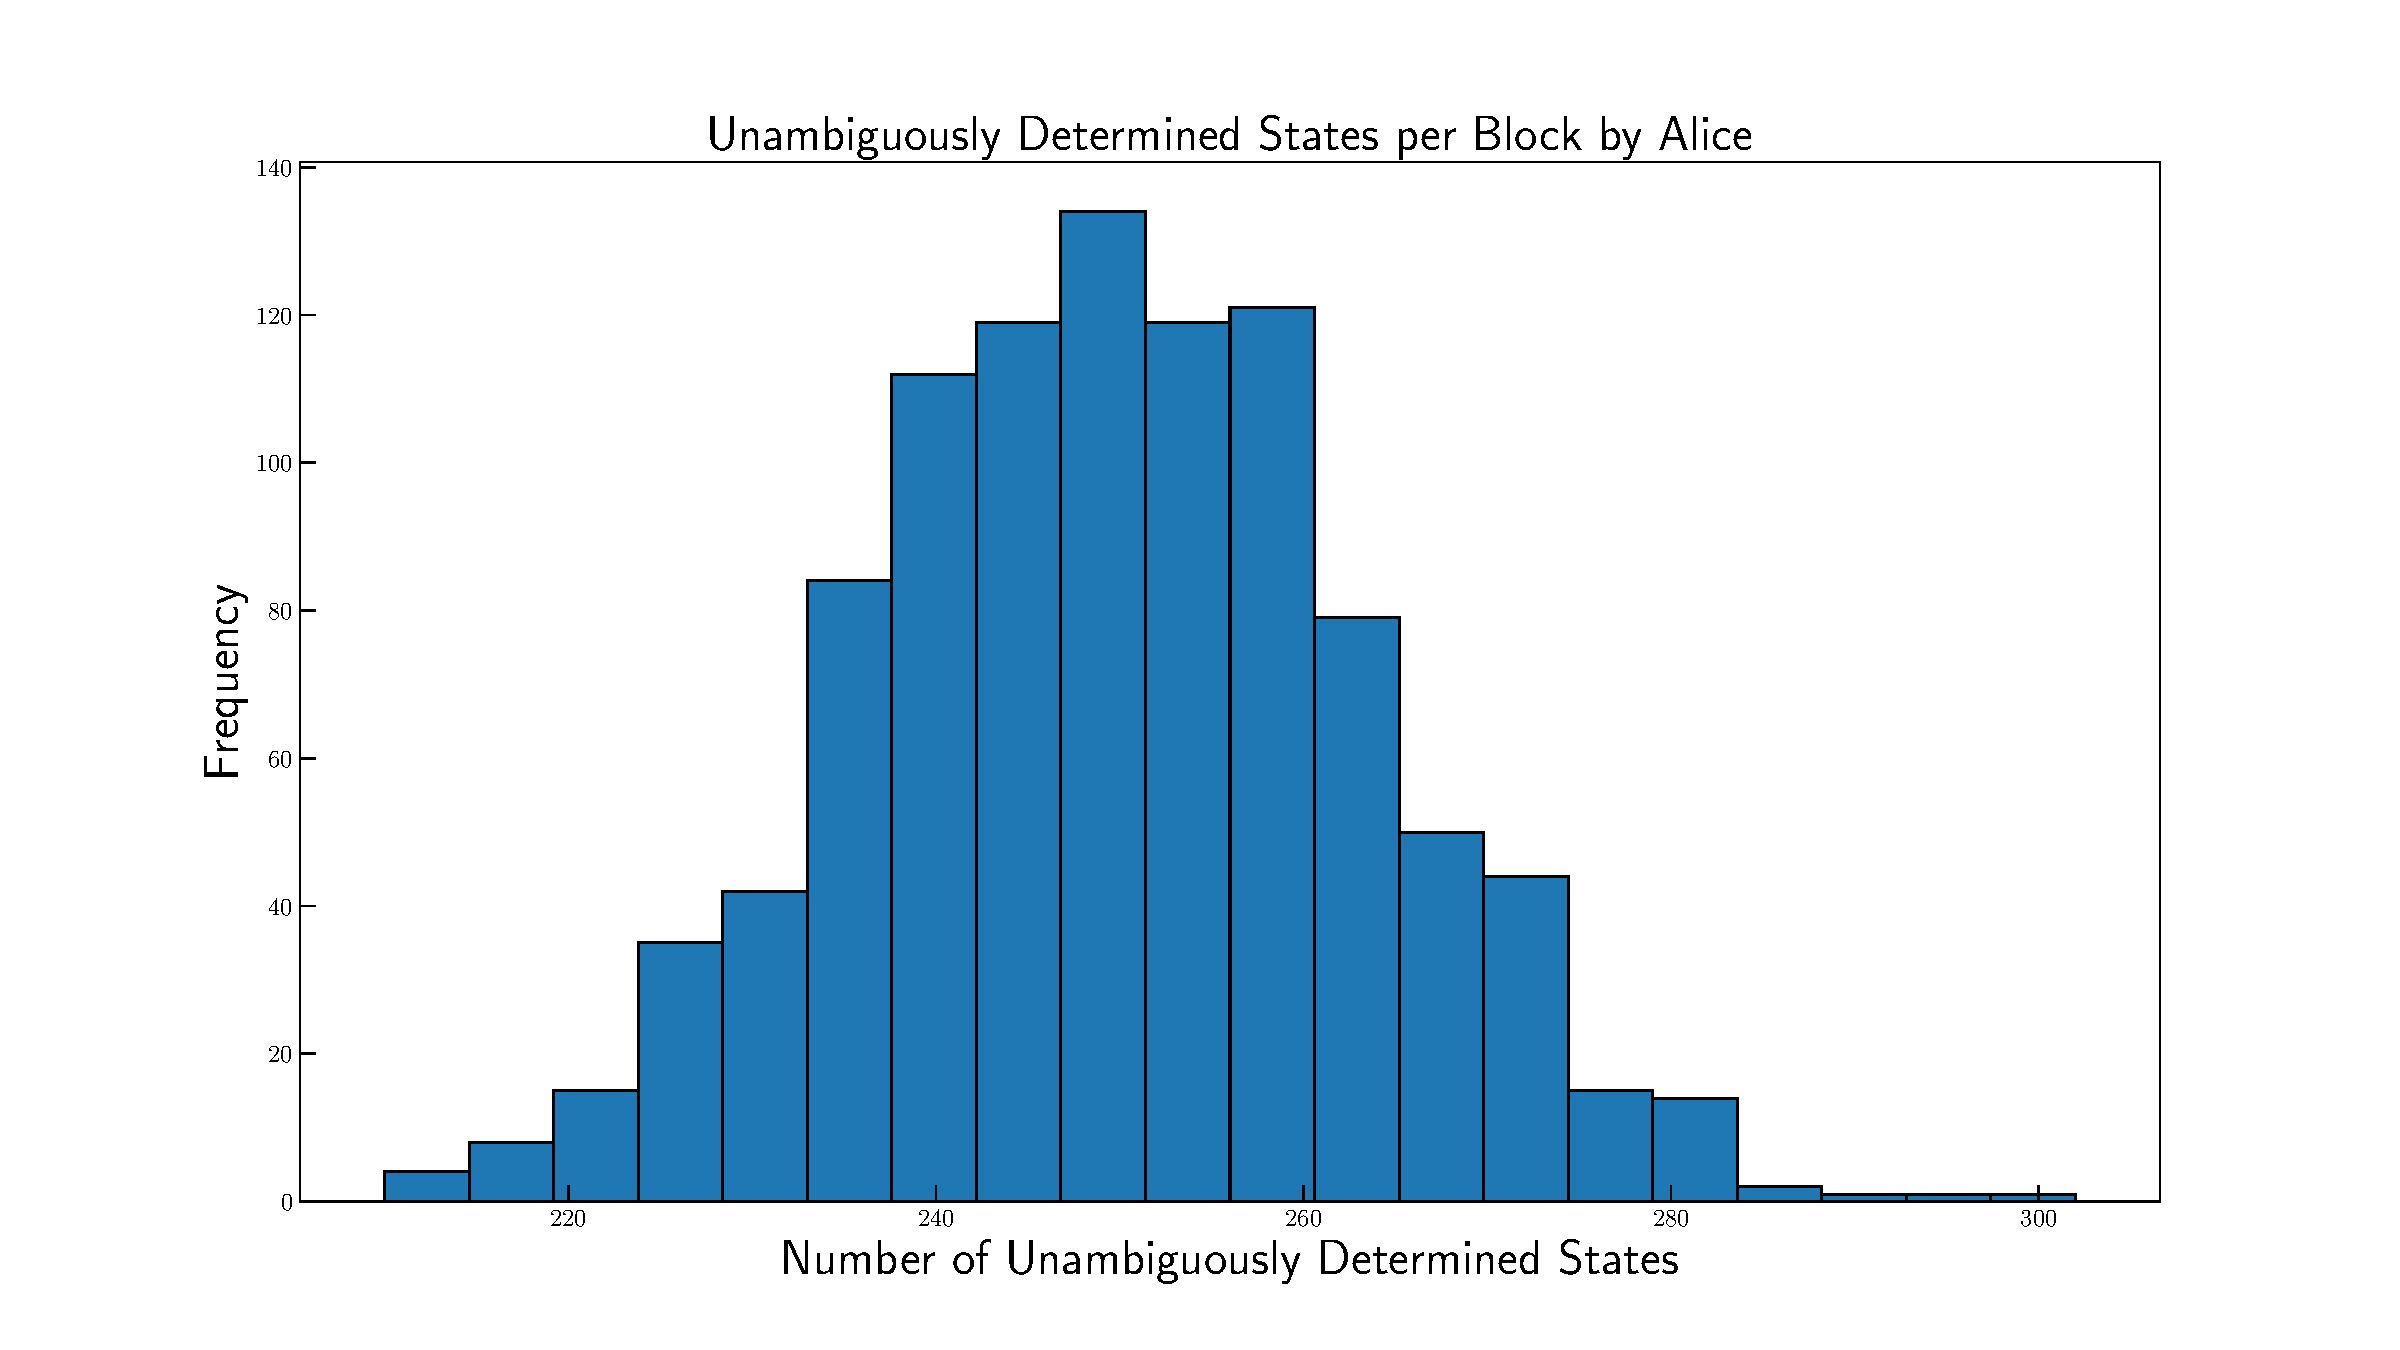
\includegraphics[width=\linewidth]{USD_number_per_block_histogram.pdf}
    \caption{The histogram showing the number of unambiguously determined states by Alice, for $n=10000, k=1000$.}
    \label{fig:USD_number_per_block_histogram}
\end{figure}
In Figure~\ref{fig:USD_number_per_block_histogram}, it shows the histogram showing the number of unambiguously determined states by Alice, for $n=10000, k=1000$ without noise, one can clearly see that the histogram peaked at around $250$, which means, most of the blocks have around $1/4$ of the states being unambiguously determined.

\begin{figure}
    \centering
    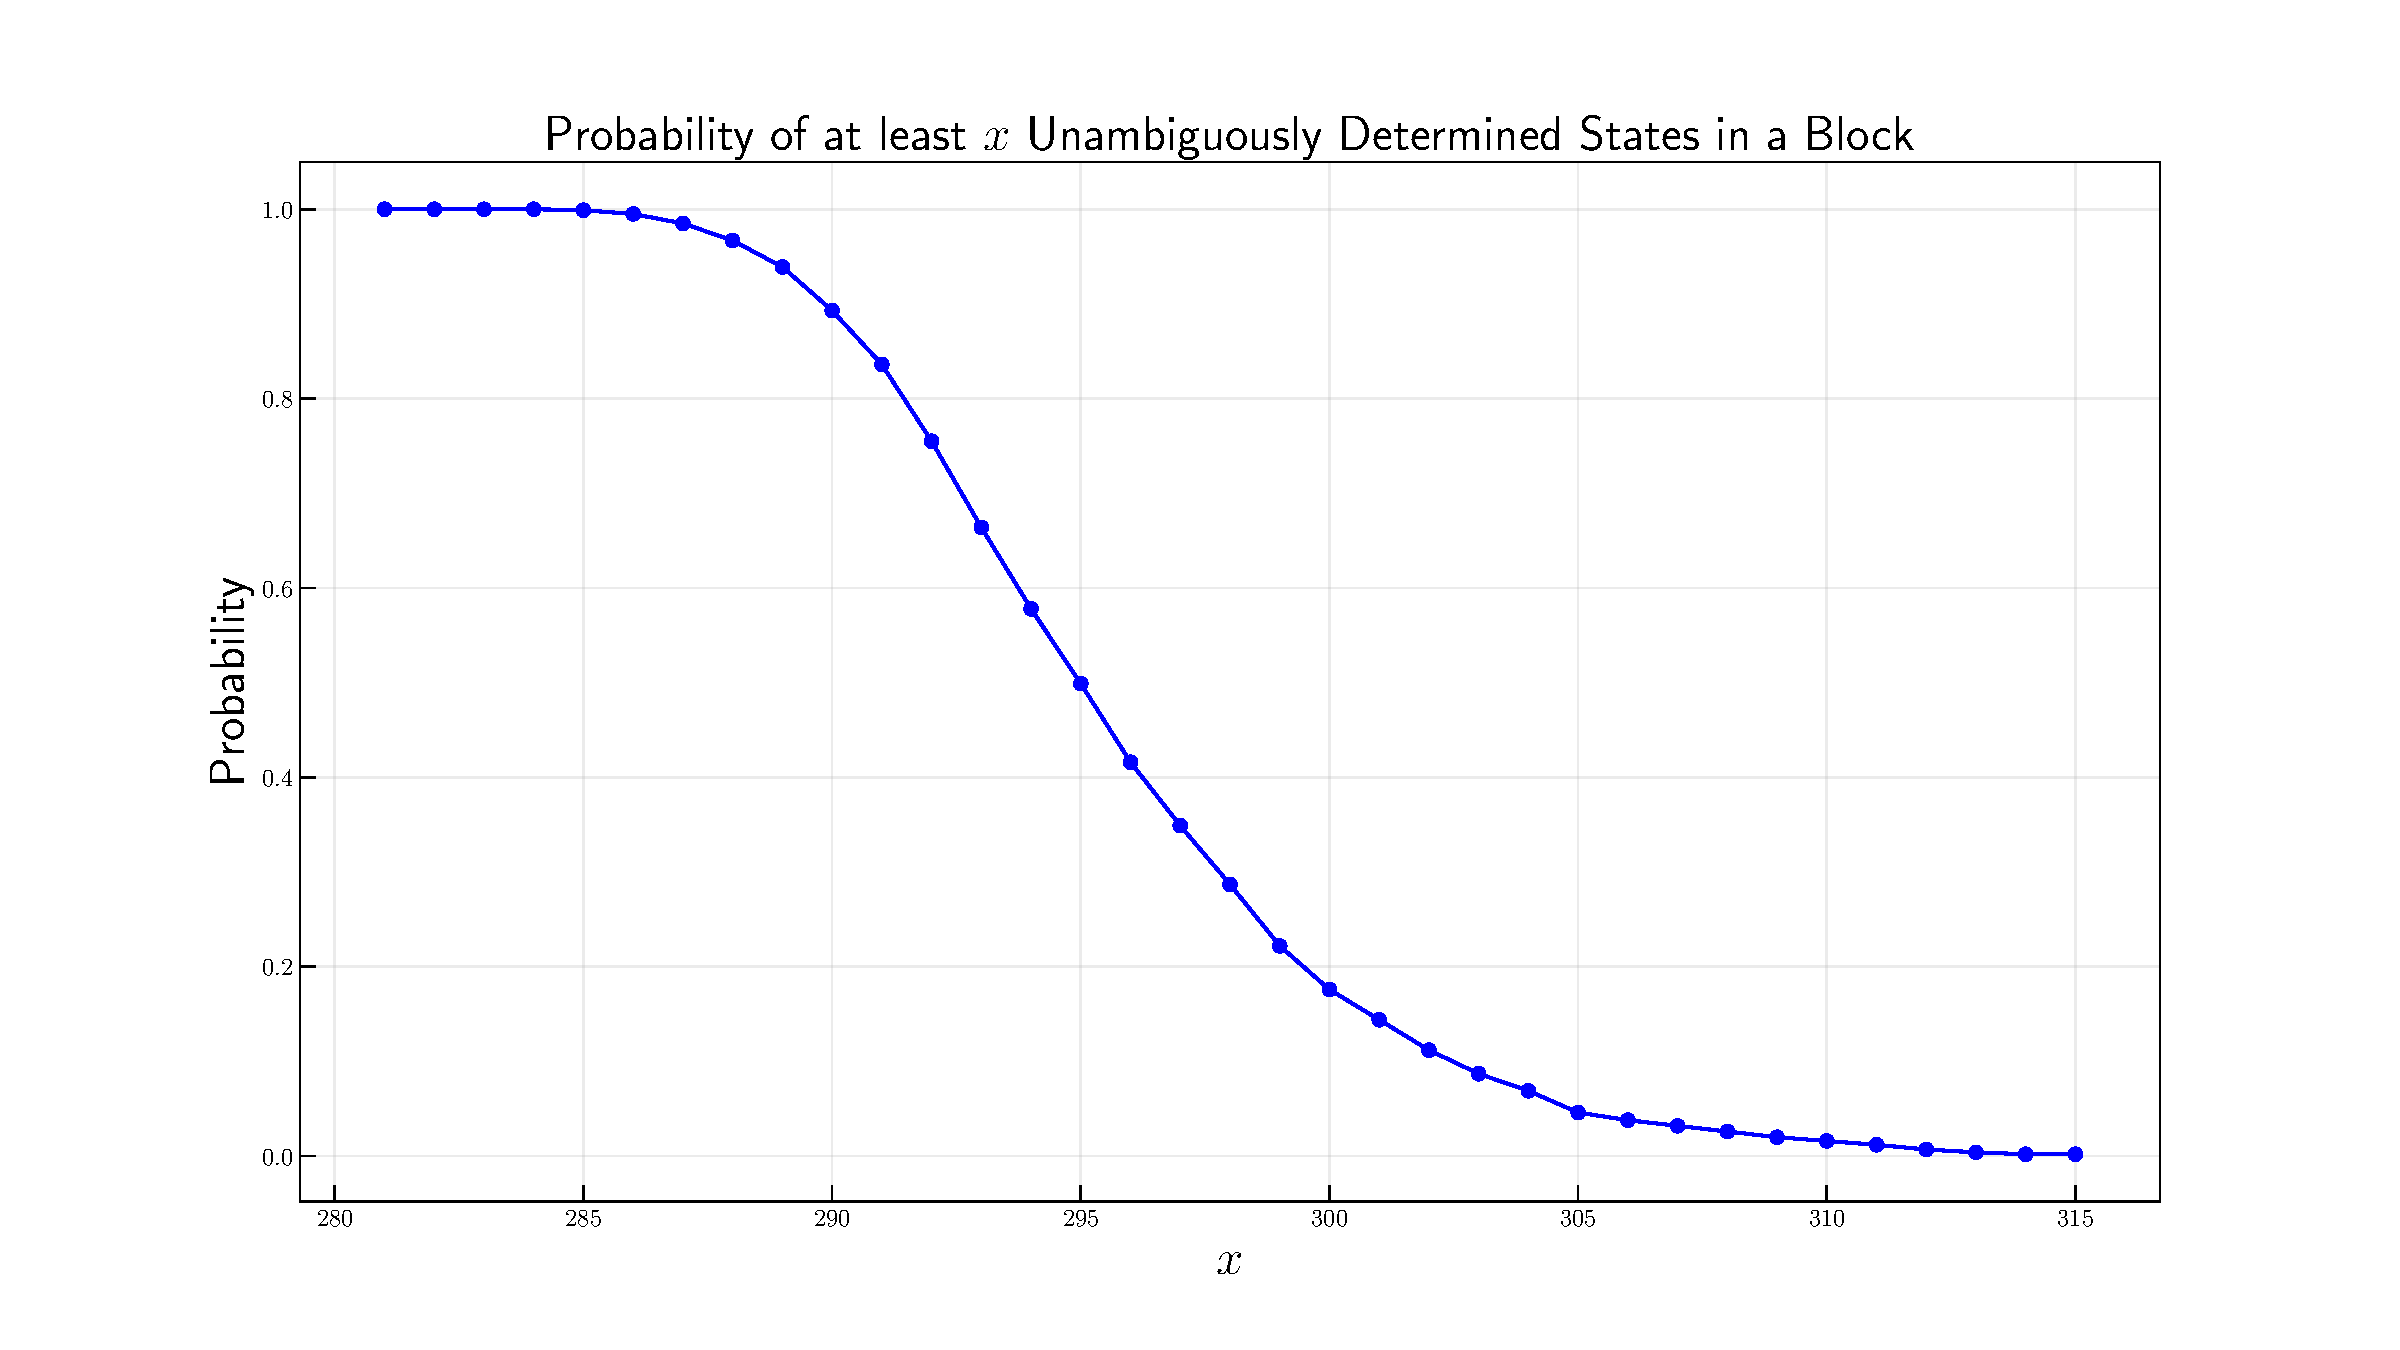
\includegraphics[width=\linewidth]{Probability_at_least_x_USD_states.pdf}
    \caption{The probability of at least $x$ unambiguously determined state in a block, calculated by running $100$ times of simulation for $n=1000, k=1000$.}
    \label{fig:Probability_at_least_x_USD_states}
\end{figure}

Figure~\ref{fig:Probability_at_least_x_USD_states} shows the probability of at least $x$ unambiguously determined state in a block, calculated by running $100$ times of simulation for $n=1000, k=1000$, the figure only shows $x\in[280, 315]$ because $p=1$ for all $x<280$ and $p=0$ for all $x>315$. One can see that the probability dropped very fast at the threshold value around $290$.

\section{Conclusion}
We conclude that...



\appendix

\section{Depolarizing and Dephasing Noise}
A quantum channel can be described by a CPTP map, which can be written in many different representations. For example, in the Kraus representation, a channel on a state $\rho$, $\mathcal{E}(\rho)$, can be written as:
\begin{equation}
    \mathcal{E}(\rho)=\sum_K \lambda_K K^\dagger\rho K
\end{equation}
where $K$ is called the Kraus operators, which satisfy 
\begin{equation}
    \sum_KK^\dagger K=I
\end{equation}
and the parameters $\lambda_K>0$.
Here, we consider the two most common types of errors, the depolarizing noise and the dephasing noise, and we explore their effect on the error rate of USD.

Recall that for a state $\rho$ and an projective operator $P$, the probability of projecting $\rho$ onto $P$ is given by
\begin{equation}
    p_{projection}(\rho, P)=Tr[\rho P]
\end{equation}

\subsection{Depolarizing Noise}
The general form of depolarizing noise with depolarizing probability $p$ on a $d$-level quantum system in Kraus representation is:
\begin{equation}
    \mathcal{E}^{depolar}_{p}(\rho)=(1-p)\rho+p\frac{I}{d}
\end{equation}

Here we consider 2-level systems without generalized measurement. We can easily check that if a state $\rho$ is originally prepared in either $\sigma_X$ or $\sigma_Z$ basis, then the state undergoes depolarization, and being measured in the complementary basis, the probability of getting either result is still $1/2$. Mathematically, 
\begin{equation}
    Tr[\mathcal{E}^{depolar}_p(\rho_0)P]=1/2
\end{equation}
for all the following combinations: $(\rho_0, P)=(\ket{0\text{ or }1}\bra{0\text{ or }1}, \ket{\pm}\bra{\pm}), (\ket{\pm}\bra{\pm}, (\ket{0\text{ or }1}\bra{0\text{ or }1})$.

Hence, if Bob prepares a state and sends it to Alice under a depolarizing channel, the probability of correctly USD is not changed. What does change is the false positive rate. For example, if Bob prepares the state $\ket{0}$, and Alice measures in $\sigma_Z$ basis and gets $\ket{1}$.

\begin{equation}
Tr[\mathcal{E}^{depolar}_p(\ket{0}\bra{0})\ket{1}\bra{1}]=p/2
\end{equation}

Which means, when Bob prepares state $\ket{0}$, and Alice measures in $\sigma_Z$, with probability $p/2$, Alice will obtain the state $\ket{1}$. Denotes $\ket{\psi}_B$ as the initial state prepared by Bob, $P_A$ as the measurement basis chosen by Alice, and $r_A\in\{+1, -1\}$ as the measurement result. This error happened to the 4 cases, $\left(\ket{\psi}_B, P_A, r_A\right)=(\ket{0},\sigma_Z, -1), (\ket{1},\sigma_Z, +1), (\ket{+},\sigma_X, -1), (\ket{-},\sigma_X, +1)$. Each of the 4 cases happens with probability $p/2$ upon the chosen of specific basis.

Hence, the probability of a state measurement being falsely considered as a successful USD:
\begin{equation}
    \text{False Positive}=\frac{1}{4}\times\frac{1}{2}\times\frac{p}{2}\times4 = \frac{p}{4}
\end{equation}

Hence, the False positive error rate:
\begin{equation}
    e_{depolar}=\frac{p/4}{1/4+p/4}=\frac{p}{1+p}
\end{equation}

\subsection{Dephasing Noise}
The general form of dephasing noise with dephasing probability in $\sigma_X$, $\sigma_Y$ and $\sigma_Z$ direction with probability $p_X, p_Y, p_Z$ on a $d$-level quantum system in Kraus representation is:
\begin{equation}
    \mathcal{E}^{dephase}_{p_x, p_y, p_z}(\rho)=(1-p_x-p_y-p_Z)\rho+\sum_{D=X, Y, Z}p_D\sigma_D\rho\sigma_D^\dagger
\end{equation}

We can easily check that if a state $\rho$ is original prepared in either $\sigma_X$ or $\sigma_Z$ basis, then the state undergoes dephasing of arbitrary noise, and being measured in the complementary basis, the probability of getting either results are still $1/2$.
\begin{equation}
    Tr[\mathcal{E}^{dephase}_{p_x, p_y, p_z}(\rho_0)P]=1/2
\end{equation}
for all the following combinations: $(\rho_0, P)=(\ket{0\text{ or }1}\bra{0\text{ or }1}, \ket{\pm}\bra{\pm}), (\ket{\pm}\bra{\pm}, (\ket{0\text{ or }1}\bra{0\text{ or }1})$.

Hence, if Bob prepares a state and sends to Alice under a dephasing channel, the probability of correctly USD is not changed. What does change is the false positive rate, For example, if Bob prepares state $\ket{0}$, and Alice measures in $\sigma_Z$ basis and gets $\ket{1}$.
\begin{equation}
Tr[\mathcal{E}^{dephase}_{p_x, p_y, p_z}(\ket{0}\bra{0})\ket{1}\bra{1}]=p_x+p_y
\end{equation}
\begin{equation}
Tr[\mathcal{E}^{dephase}_{p_x, p_y, p_z}(\ket{1}\bra{1})\ket{0}\bra{0}]=p_x+p_y
\end{equation}
\begin{equation}
Tr[\mathcal{E}^{dephase}_{p_x, p_y, p_z}(\ket{+}\bra{+})\ket{-}\bra{-}]=p_y+p_z
\end{equation}
\begin{equation}
Tr[\mathcal{E}^{dephase}_{p_x, p_y, p_z}(\ket{-}\bra{-})\ket{+}\bra{+}]=p_y+p_z
\end{equation}

Hence, the probability of a state measurement being falsely considered as a successful USD:
\begin{equation}
\begin{split}
    \text{False Positive}&=\frac{1}{4}\times\frac{1}{2}\times\left(2p_x+2p_y+2p_y+2p_z\right)\\
    &=\frac{p_x+2p_y+p_z}{4}
    \end{split}
\end{equation}

Hence, the False positive error rate:
\begin{equation}
    e_{depolar}=\frac{\frac{p_x+2p_y+p_z}{4}}{1/4+\frac{p_x+2p_y+p_z}{4}}=\frac{p_x+2p_y+p_z}{1+p_x+2p_y+p_z}
\end{equation}




\bibliography{SPIR_Single_Database}% Produces the bibliography via BibTeX.

\end{document}
%
% ****** End of file apssamp.tex ******
